\begin{figure}
\centering
	% To include a figure from a file named example.*
	% Allowable file formats are eps or ps if compiling using latex
	% or pdf, png, jpg if compiling using pdflatex
	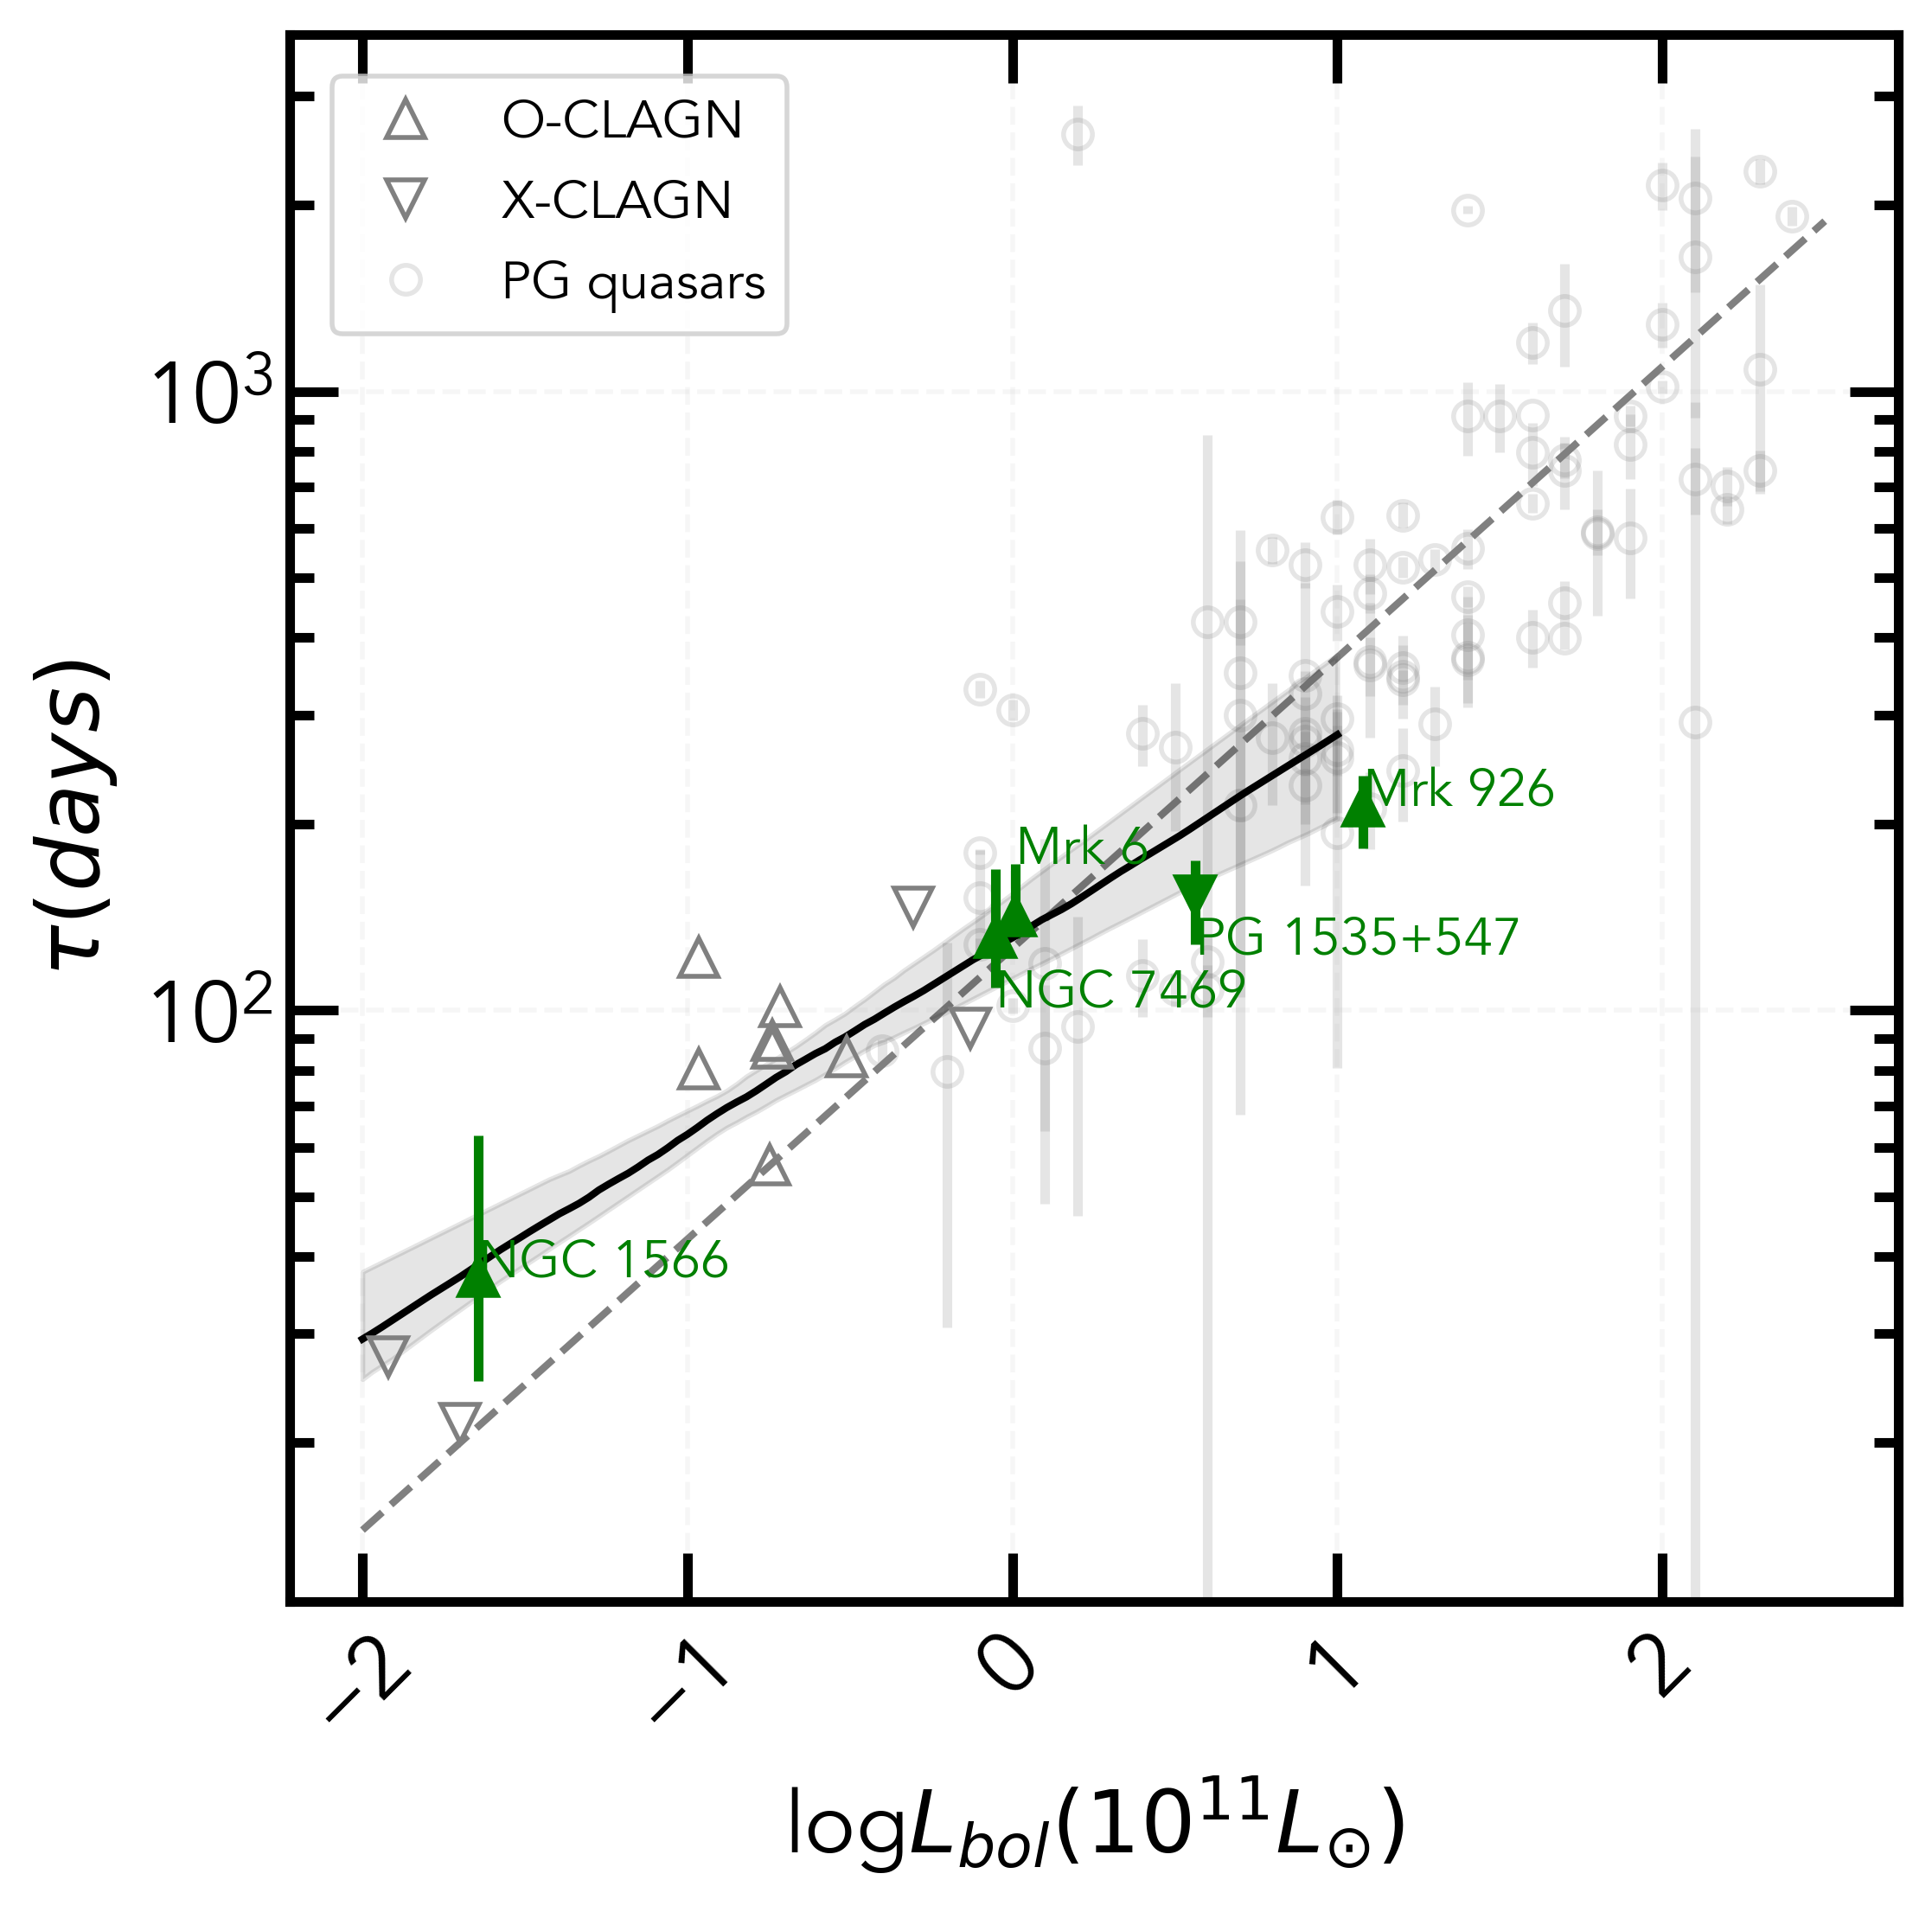
\includegraphics[width=0.45\textwidth]{tau_L_correlation_clagn.png}
    \caption{$\tau$-L correlation for CLAGNs, where $\tau$ is time lag between V band and $W$1 band and L is bolometric luminosity. Grey circles represent PG quasars \citep{2019ApJ...886...33L} for comparison. The dashed line repserent the best fitting of $\tau$-L correlation for PG quasars in \citet{2019ApJ...886...33L}. The straight line is the best fitting for CLAGNs with a scatter in the shadow region.} 
    \label{fig:tau_L}
\end{figure}


\begin{table}
 \caption{Dust reverberation time lag of CLAGNs.
}
 \label{table_lag}
 \begin{center}
 \begin{tabular}{lcccc}
 \hline\hline
Name & log($L_{bol}$) & $\tau$~(days) &Type \\ \hline 
Mrk 590 & 44.13 & $57.9^{+17.8}_{-20.0}$ & O \\
Mrk 6 & 44.59 & $142.1^{+30.0}_{-11.5}$ & O \\
Mrk 926 & 45.66 & $213.8^{+25.3}_{-31.0}$ & O \\
NGC 1566 & 42.94 & $37.1^{+25.7}_{-11.9}$ & O \\
NGC 3516 & 44.19 & $91.1^{+64.0}_{-31.4}$ & O \\
NGC 4051 & 42.61 & $22.3^{+10.4}_{-10.0}$ & X \\
NGC 4151 & 44.08 & $74.4^{+40.8}_{-19.5}$ & O \\
NGC 5548 & 44.66 & $131.2^{+18.6}_{-32.2}$ & O \\
NGC 7469 & 44.53 & $131.2^{+37.9}_{-22.4}$ & X \\
PG 1535+547 & 45.15 & $153.2^{+21.2}_{-25.3}$ & X \\
\hline\hline
\end{tabular}
\end{center}
Note. The table lists source name, bolometric luminosity, dust reverberation time lag between V band and $W$1 band, CLAGN types (``O'' for optical CLAGN and ``X'' for X-ray CLAGN). 
\end{table}

